%!TEX encoding = UTF-8 Unicode

%!TEX root = ../compendium.tex

\Lab{\LabWeekSEVEN}

\begin{Goals}
\item Kunna arv
\item Kunna traits
\end{Goals}

\begin{Preparations}
\item Gör övning {\tt \ExeWeekSEVEN} i kapitel \ref{exe:W07}.
\item Läs på om och förstå arv
\end{Preparations}

\subsection{Bakgrund}
I labben kommer sköldpaddor, \code{Turtle}, att får tävla mot varandra i ett lopp. Racet kommer att köras i ett \code{RaceWindow} som ärver från \code{SimpleWindow}. Först kommer en \code{RaceTurtle} att skapas, som ärver från \code{Turtle} och sen kommer sköldpaddor med olika egenskaper skapas. Dessa sköldpaddor kommer sen att tävla i en tunering med 32 sköldpaddor. Det kommer vara åtta sköldpaddor i varje deltävling och tuneringen kommer bestå av fyra kvartsfinaler, två semifinaler och tillsist en final.

\subsection{Obligatoriska uppgifter}

\Task \code{RaceWindow}

\Subtask Skapa \code{RaceWindow} som ärver från \code{SimpleWindow} med fix storlek och förbestämd titel. Lämplig storlek är 800x400. Det ska finnas två attribut \code{startX} och \code{endX} som är förbestämda och motsvarar start och mål.

\Subtask Skapa tre metoder \code{startX}, \code{endX} och \code{startY}. \code{startX} och \code{endX} ska retunera värdet på motsvarande attribut. \code{startY} ska ta in ett heltal \code{nbr} som är ett startnummer och retunera y-värdet för det startnumret. \code{startX} och \code{endX} är x-värdet för start- resp. målinjen och \code{startY} är y-värdet för varje sköldpaddas startposition på startlinjen.

\Subtask Skapa en metod \code{draw} som ritar upp ett race i fönstret och skriver ut startnummer. Definiera gärna en klass som ritar upp ett start-/målfält. Bilden är enbart ett exempel på vad man kan göra. Rita något kul! Titeln och alla tävlande turtles kommer att skrivas ut senare i uppgiften.

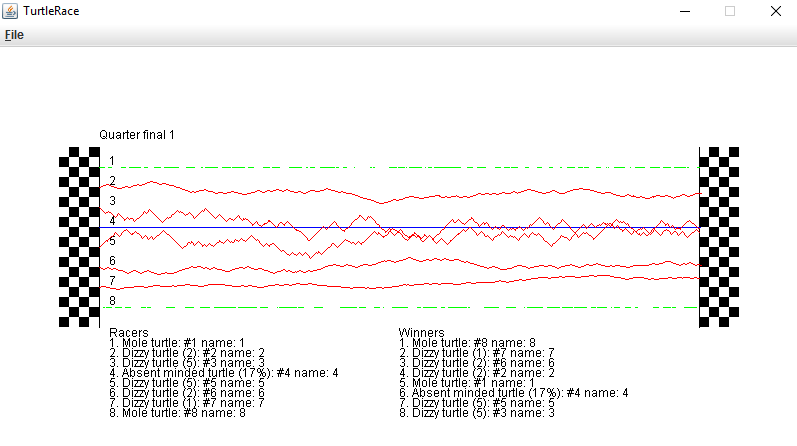
\includegraphics[width=\textwidth]{../img/turtlerace/RaceWindow}

\Subtask Skapa en metod \code{printTitle} som tar in en sträng och skriver ut den som titel på racet.

\begin{Code}
class RaceTurtle(private val w: RaceWindow,
			var nbr: Int, val name: String) {
  /**
   * Takes one step of a random length 1 to 5
   */
  def raceStep(): Unit = ???

  /**
   * Restarts the turtle at the finish line.
   * To be used before each race
   */
  def restart: Unit = ???

  override def toString: String = ???
}
\end{Code}

\Task \code{RaceTurtle}.

\Subtask Högerklicka på projektet \code{w07_turtlerace_team} och välj \code{Build Path} $\rightarrow$ \code{Configure Build Path}. Välj fliken \code{Projects} och tryck \code{Add...}. Markera projektet \code{w06_turtlegraphics} och tryck \code{OK}.

\Subtask Implementera klassen \code{RaceTurtle} som ska ärva från \code{Turtle}. \code{Turtle} och \code{Point} behöver importeras från \code{turtlegraphics}. Startpositionen för en \code{RaceTurtle} hämtas från \code{RaceWindow}.\\Exempel på import-sats: \code{import turtlegraphics.Turtle}.

\Subtask Skapa en metod \code{printRacers}, i \code{RaceWindow}, som tar in en lista med \code{RaceTurtle}, ett $x$-värde och en titel på listan och skriver ut listan med början på angivet $x$-värde. Se exemplet med listan \textit{Racers} och \textit{Winners}.

\Task \code{TurtleRace}

\Subtask Implementera metoden \code{race} som ska börja med att skriva ut tävlande och titel i \code{RaceWindow}. Skapa en tom \code{ArrayBuffer} med namnet \code{winners} (för detta behöver man importera \code{scala.collection.mutable.ArrayBuffer}). Låt varje \code{RaceTurtle} ta ett steg tills en passerar mållinjen. Lägg över alla som passerat mållinjen i \code{winners} och kör detta tills alla \code{RaceTurtle} har hamnat i \code{winners}. Använd \code{SimpleWindow.delay(5)} mellan varje steg för att se animeringen. Skriv ut vinnarna i \code{RaceWindow} och vänta på musklick. Retunera listan med vinnare.

\Subtask Testa att köra ett race mellan åtta sköldpaddor.

\Task \code{ColorTurtle}.

\Subtask Skapa en ny klass \code{ColorTurtle} som ärver från \code{RaceTurtle} och tar in en extra parameter \code{color} av typen \code{java.awt.Color}.

\Subtask Metoden \code{raceStep} är det enda som skiljer klasserna. Börja med att spara undan nuvarande färg i \code{RaceWindow} och byt till den angivna färgen \code{color}. Anropa \code{raceStep} i superklassen och ändra sedan tillbaka färgen i \code{RaceWindow}.

\Task \code{Dizziness}, \code{AbsentMindness} och \code{Mole}

\Subtask Implementera tre \code{trait} som ärver från \code{RaceTurtle} och som \code{override} \code{raceStep} och \code{toString}. \code{toString} ska utöver \code{toString} från \code{RaceTurtle} även bestå av vilken typ av \code{RaceTurtle} det är och graden av yrsel/tankspriddhet den har.

\begin{itemize}

\item \code{Dizziness}. Slumpa ett heltal \code{dizziness} mellan 1 och 5. För varje steg ska en riktningsförändring slumpas fram som blir större desto större \code{dizziness} är. Slumpa även om den avviker åt höger eller vänster och använd \code{turnRight} och \code{turnLeft}.

\item \code{AbsentMindness}. Slumpa ett heltal \code{absent} mellan 0 och 99 som anger i procent hur tankspridd \code{RaceTurtle} är. För varje steg ska det vara \code{absent}\% chans att ett steg inte tas.

\item \code{Mole}. Med 50\% sannolikhet ska denna typ \code{RaceTurtle} gräva ner sig i marken. För varje steg ska det vara 50\% chans att pennan är uppe och 50\% chans att pennan är nere. Använd metoderna \code{penUp} och \code{penDown}.

\end{itemize}

\Task \code{TurtleTournament}

\Subtask Börja med att skapa en hjälpmetod \code{randTurtle} som tar in ett \code{RaceWindow}, ett nummer och ett namn som parameter. Slumpa med lika stor sannolikhet mellan att skapa en \code{ColorTurtle} med en av de tre olika egenskaperna och låt de olika egenskaperna ha olika färger.

\Subtask Skapa ett \code{RaceWindow}. Slumpa fram 32 sköldpaddor och låt dem utföra fyra \code{TurtleRace}. Ta vara på vinnarna och låta de fyra bästa från varja lopp köra två lopp till. De fyra bästa från båda dessa loppen går vidare till finalen. \textbf{Tänk på att rensa \code{RaceWindow} efter varje lopp och rita ut det på nytt innan varje lopp}.
